% GNUPLOT: LaTeX picture with Postscript
\begingroup
  \makeatletter
  \providecommand\color[2][]{%
    \GenericError{(gnuplot) \space\space\space\@spaces}{%
      Package color not loaded in conjunction with
      terminal option `colourtext'%
    }{See the gnuplot documentation for explanation.%
    }{Either use 'blacktext' in gnuplot or load the package
      color.sty in LaTeX.}%
    \renewcommand\color[2][]{}%
  }%
  \providecommand\includegraphics[2][]{%
    \GenericError{(gnuplot) \space\space\space\@spaces}{%
      Package graphicx or graphics not loaded%
    }{See the gnuplot documentation for explanation.%
    }{The gnuplot epslatex terminal needs graphicx.sty or graphics.sty.}%
    \renewcommand\includegraphics[2][]{}%
  }%
  \providecommand\rotatebox[2]{#2}%
  \@ifundefined{ifGPcolor}{%
    \newif\ifGPcolor
    \GPcolortrue
  }{}%
  \@ifundefined{ifGPblacktext}{%
    \newif\ifGPblacktext
    \GPblacktexttrue
  }{}%
  % define a \g@addto@macro without @ in the name:
  \let\gplgaddtomacro\g@addto@macro
  % define empty templates for all commands taking text:
  \gdef\gplbacktext{}%
  \gdef\gplfronttext{}%
  \makeatother
  \ifGPblacktext
    % no textcolor at all
    \def\colorrgb#1{}%
    \def\colorgray#1{}%
  \else
    % gray or color?
    \ifGPcolor
      \def\colorrgb#1{\color[rgb]{#1}}%
      \def\colorgray#1{\color[gray]{#1}}%
      \expandafter\def\csname LTw\endcsname{\color{white}}%
      \expandafter\def\csname LTb\endcsname{\color{black}}%
      \expandafter\def\csname LTa\endcsname{\color{black}}%
      \expandafter\def\csname LT0\endcsname{\color[rgb]{1,0,0}}%
      \expandafter\def\csname LT1\endcsname{\color[rgb]{0,1,0}}%
      \expandafter\def\csname LT2\endcsname{\color[rgb]{0,0,1}}%
      \expandafter\def\csname LT3\endcsname{\color[rgb]{1,0,1}}%
      \expandafter\def\csname LT4\endcsname{\color[rgb]{0,1,1}}%
      \expandafter\def\csname LT5\endcsname{\color[rgb]{1,1,0}}%
      \expandafter\def\csname LT6\endcsname{\color[rgb]{0,0,0}}%
      \expandafter\def\csname LT7\endcsname{\color[rgb]{1,0.3,0}}%
      \expandafter\def\csname LT8\endcsname{\color[rgb]{0.5,0.5,0.5}}%
    \else
      % gray
      \def\colorrgb#1{\color{black}}%
      \def\colorgray#1{\color[gray]{#1}}%
      \expandafter\def\csname LTw\endcsname{\color{white}}%
      \expandafter\def\csname LTb\endcsname{\color{black}}%
      \expandafter\def\csname LTa\endcsname{\color{black}}%
      \expandafter\def\csname LT0\endcsname{\color{black}}%
      \expandafter\def\csname LT1\endcsname{\color{black}}%
      \expandafter\def\csname LT2\endcsname{\color{black}}%
      \expandafter\def\csname LT3\endcsname{\color{black}}%
      \expandafter\def\csname LT4\endcsname{\color{black}}%
      \expandafter\def\csname LT5\endcsname{\color{black}}%
      \expandafter\def\csname LT6\endcsname{\color{black}}%
      \expandafter\def\csname LT7\endcsname{\color{black}}%
      \expandafter\def\csname LT8\endcsname{\color{black}}%
    \fi
  \fi
  \setlength{\unitlength}{0.0500bp}%
  \begin{picture}(8206.00,11520.00)%
      \csname LTb\endcsname%
      \put(4103,11300){\makebox(0,0){\strut{}Referenzspektren Teil 1}}%
    \gplgaddtomacro\gplbacktext{%
      \csname LTb\endcsname%
      \put(688,7776){\makebox(0,0)[r]{\strut{}0}}%
      \csname LTb\endcsname%
      \put(688,8304){\makebox(0,0)[r]{\strut{}100}}%
      \csname LTb\endcsname%
      \put(688,8832){\makebox(0,0)[r]{\strut{}200}}%
      \csname LTb\endcsname%
      \put(688,9359){\makebox(0,0)[r]{\strut{}300}}%
      \csname LTb\endcsname%
      \put(688,9887){\makebox(0,0)[r]{\strut{}400}}%
      \csname LTb\endcsname%
      \put(688,10415){\makebox(0,0)[r]{\strut{}500}}%
      \csname LTb\endcsname%
      \put(688,10943){\makebox(0,0)[r]{\strut{}600}}%
      \csname LTb\endcsname%
      \put(820,7556){\makebox(0,0){\strut{} }}%
      \csname LTb\endcsname%
      \put(1382,7556){\makebox(0,0){\strut{} }}%
      \csname LTb\endcsname%
      \put(1944,7556){\makebox(0,0){\strut{} }}%
      \csname LTb\endcsname%
      \put(2506,7556){\makebox(0,0){\strut{} }}%
      \csname LTb\endcsname%
      \put(3068,7556){\makebox(0,0){\strut{} }}%
      \csname LTb\endcsname%
      \put(3630,7556){\makebox(0,0){\strut{} }}%
      \put(50,9359){\rotatebox{-270}{\makebox(0,0){\strut{}Counts}}}%
      \put(3347,10690){\makebox(0,0)[l]{\strut{}Pb}}%
    }%
    \gplgaddtomacro\gplfronttext{%
    }%
    \gplgaddtomacro\gplbacktext{%
      \csname LTb\endcsname%
      \put(4381,7776){\makebox(0,0)[r]{\strut{}0}}%
      \csname LTb\endcsname%
      \put(4381,8093){\makebox(0,0)[r]{\strut{}1000}}%
      \csname LTb\endcsname%
      \put(4381,8409){\makebox(0,0)[r]{\strut{}2000}}%
      \csname LTb\endcsname%
      \put(4381,8726){\makebox(0,0)[r]{\strut{}3000}}%
      \csname LTb\endcsname%
      \put(4381,9043){\makebox(0,0)[r]{\strut{}4000}}%
      \csname LTb\endcsname%
      \put(4381,9359){\makebox(0,0)[r]{\strut{}5000}}%
      \csname LTb\endcsname%
      \put(4381,9676){\makebox(0,0)[r]{\strut{}6000}}%
      \csname LTb\endcsname%
      \put(4381,9993){\makebox(0,0)[r]{\strut{}7000}}%
      \csname LTb\endcsname%
      \put(4381,10310){\makebox(0,0)[r]{\strut{}8000}}%
      \csname LTb\endcsname%
      \put(4381,10626){\makebox(0,0)[r]{\strut{}9000}}%
      \csname LTb\endcsname%
      \put(4381,10943){\makebox(0,0)[r]{\strut{}10000}}%
      \csname LTb\endcsname%
      \put(4513,7556){\makebox(0,0){\strut{} }}%
      \csname LTb\endcsname%
      \put(5075,7556){\makebox(0,0){\strut{} }}%
      \csname LTb\endcsname%
      \put(5637,7556){\makebox(0,0){\strut{} }}%
      \csname LTb\endcsname%
      \put(6199,7556){\makebox(0,0){\strut{} }}%
      \csname LTb\endcsname%
      \put(6760,7556){\makebox(0,0){\strut{} }}%
      \csname LTb\endcsname%
      \put(7322,7556){\makebox(0,0){\strut{} }}%
      \put(7039,10690){\makebox(0,0)[l]{\strut{}Fe}}%
    }%
    \gplgaddtomacro\gplfronttext{%
    }%
    \gplgaddtomacro\gplbacktext{%
      \csname LTb\endcsname%
      \put(688,4320){\makebox(0,0)[r]{\strut{}0}}%
      \csname LTb\endcsname%
      \put(688,4672){\makebox(0,0)[r]{\strut{}50}}%
      \csname LTb\endcsname%
      \put(688,5024){\makebox(0,0)[r]{\strut{}100}}%
      \csname LTb\endcsname%
      \put(688,5376){\makebox(0,0)[r]{\strut{}150}}%
      \csname LTb\endcsname%
      \put(688,5728){\makebox(0,0)[r]{\strut{}200}}%
      \csname LTb\endcsname%
      \put(688,6079){\makebox(0,0)[r]{\strut{}250}}%
      \csname LTb\endcsname%
      \put(688,6431){\makebox(0,0)[r]{\strut{}300}}%
      \csname LTb\endcsname%
      \put(688,6783){\makebox(0,0)[r]{\strut{}350}}%
      \csname LTb\endcsname%
      \put(688,7135){\makebox(0,0)[r]{\strut{}400}}%
      \csname LTb\endcsname%
      \put(688,7487){\makebox(0,0)[r]{\strut{}450}}%
      \csname LTb\endcsname%
      \put(820,4100){\makebox(0,0){\strut{} }}%
      \csname LTb\endcsname%
      \put(1382,4100){\makebox(0,0){\strut{} }}%
      \csname LTb\endcsname%
      \put(1944,4100){\makebox(0,0){\strut{} }}%
      \csname LTb\endcsname%
      \put(2506,4100){\makebox(0,0){\strut{} }}%
      \csname LTb\endcsname%
      \put(3068,4100){\makebox(0,0){\strut{} }}%
      \csname LTb\endcsname%
      \put(3630,4100){\makebox(0,0){\strut{} }}%
      \put(50,5903){\rotatebox{-270}{\makebox(0,0){\strut{}Counts}}}%
      \put(3347,7234){\makebox(0,0)[l]{\strut{}Au}}%
    }%
    \gplgaddtomacro\gplfronttext{%
    }%
    \gplgaddtomacro\gplbacktext{%
      \csname LTb\endcsname%
      \put(4381,4320){\makebox(0,0)[r]{\strut{}0}}%
      \csname LTb\endcsname%
      \put(4381,4672){\makebox(0,0)[r]{\strut{}20}}%
      \csname LTb\endcsname%
      \put(4381,5024){\makebox(0,0)[r]{\strut{}40}}%
      \csname LTb\endcsname%
      \put(4381,5376){\makebox(0,0)[r]{\strut{}60}}%
      \csname LTb\endcsname%
      \put(4381,5728){\makebox(0,0)[r]{\strut{}80}}%
      \csname LTb\endcsname%
      \put(4381,6079){\makebox(0,0)[r]{\strut{}100}}%
      \csname LTb\endcsname%
      \put(4381,6431){\makebox(0,0)[r]{\strut{}120}}%
      \csname LTb\endcsname%
      \put(4381,6783){\makebox(0,0)[r]{\strut{}140}}%
      \csname LTb\endcsname%
      \put(4381,7135){\makebox(0,0)[r]{\strut{}160}}%
      \csname LTb\endcsname%
      \put(4381,7487){\makebox(0,0)[r]{\strut{}180}}%
      \csname LTb\endcsname%
      \put(4513,4100){\makebox(0,0){\strut{} }}%
      \csname LTb\endcsname%
      \put(5075,4100){\makebox(0,0){\strut{} }}%
      \csname LTb\endcsname%
      \put(5637,4100){\makebox(0,0){\strut{} }}%
      \csname LTb\endcsname%
      \put(6199,4100){\makebox(0,0){\strut{} }}%
      \csname LTb\endcsname%
      \put(6760,4100){\makebox(0,0){\strut{} }}%
      \csname LTb\endcsname%
      \put(7322,4100){\makebox(0,0){\strut{} }}%
      \put(7039,7234){\makebox(0,0)[l]{\strut{}In}}%
    }%
    \gplgaddtomacro\gplfronttext{%
    }%
    \gplgaddtomacro\gplbacktext{%
      \csname LTb\endcsname%
      \put(688,863){\makebox(0,0)[r]{\strut{}0}}%
      \csname LTb\endcsname%
      \put(688,1259){\makebox(0,0)[r]{\strut{}500}}%
      \csname LTb\endcsname%
      \put(688,1655){\makebox(0,0)[r]{\strut{}1000}}%
      \csname LTb\endcsname%
      \put(688,2051){\makebox(0,0)[r]{\strut{}1500}}%
      \csname LTb\endcsname%
      \put(688,2447){\makebox(0,0)[r]{\strut{}2000}}%
      \csname LTb\endcsname%
      \put(688,2843){\makebox(0,0)[r]{\strut{}2500}}%
      \csname LTb\endcsname%
      \put(688,3239){\makebox(0,0)[r]{\strut{}3000}}%
      \csname LTb\endcsname%
      \put(688,3635){\makebox(0,0)[r]{\strut{}3500}}%
      \csname LTb\endcsname%
      \put(688,4031){\makebox(0,0)[r]{\strut{}4000}}%
      \csname LTb\endcsname%
      \put(820,643){\makebox(0,0){\strut{} }}%
      \csname LTb\endcsname%
      \put(1382,643){\makebox(0,0){\strut{} }}%
      \csname LTb\endcsname%
      \put(1944,643){\makebox(0,0){\strut{} }}%
      \csname LTb\endcsname%
      \put(2506,643){\makebox(0,0){\strut{} }}%
      \csname LTb\endcsname%
      \put(3068,643){\makebox(0,0){\strut{} }}%
      \csname LTb\endcsname%
      \put(3630,643){\makebox(0,0){\strut{} }}%
      \put(-82,2447){\rotatebox{-270}{\makebox(0,0){\strut{}Counts}}}%
      \put(2256,313){\makebox(0,0){\strut{}x}}%
      \put(3347,3778){\makebox(0,0)[l]{\strut{}Cu}}%
    }%
    \gplgaddtomacro\gplfronttext{%
    }%
    \gplgaddtomacro\gplbacktext{%
      \csname LTb\endcsname%
      \put(4381,863){\makebox(0,0)[r]{\strut{}0}}%
      \csname LTb\endcsname%
      \put(4381,1391){\makebox(0,0)[r]{\strut{}1000}}%
      \csname LTb\endcsname%
      \put(4381,1919){\makebox(0,0)[r]{\strut{}2000}}%
      \csname LTb\endcsname%
      \put(4381,2447){\makebox(0,0)[r]{\strut{}3000}}%
      \csname LTb\endcsname%
      \put(4381,2975){\makebox(0,0)[r]{\strut{}4000}}%
      \csname LTb\endcsname%
      \put(4381,3503){\makebox(0,0)[r]{\strut{}5000}}%
      \csname LTb\endcsname%
      \put(4381,4031){\makebox(0,0)[r]{\strut{}6000}}%
      \csname LTb\endcsname%
      \put(4513,643){\makebox(0,0){\strut{} }}%
      \csname LTb\endcsname%
      \put(5075,643){\makebox(0,0){\strut{} }}%
      \csname LTb\endcsname%
      \put(5637,643){\makebox(0,0){\strut{} }}%
      \csname LTb\endcsname%
      \put(6199,643){\makebox(0,0){\strut{} }}%
      \csname LTb\endcsname%
      \put(6760,643){\makebox(0,0){\strut{} }}%
      \csname LTb\endcsname%
      \put(7322,643){\makebox(0,0){\strut{} }}%
      \put(5948,313){\makebox(0,0){\strut{}x}}%
      \put(7039,3778){\makebox(0,0)[l]{\strut{}Ni}}%
    }%
    \gplgaddtomacro\gplfronttext{%
    }%
    \gplbacktext
    \put(0,0){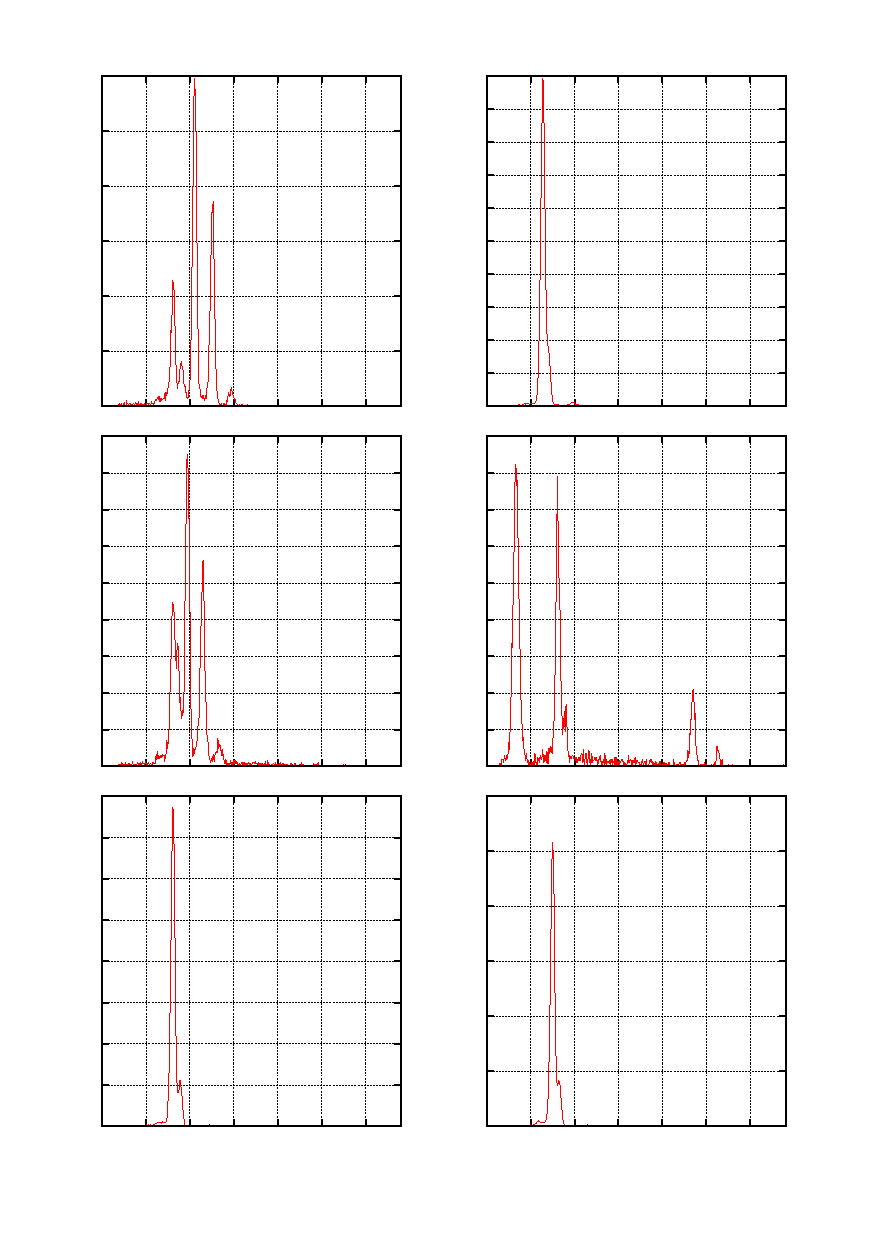
\includegraphics{./plots/referenzspektren1}}%
    \gplfronttext
  \end{picture}%
\endgroup
